\documentclass[notes]{subfiles}

\begin{document}
	\addcontentsline{toc}{section}{1.4 - The Tangent and Velocity Problems}
	\refstepcounter{section}
	\fancyhead[RO,LE]{\bfseries \large\nameref{cs14}} 
	\fancyhead[LO,RE]{\bfseries \currentname}
	\fancyfoot[C]{{}}
	\fancyfoot[RO,LE]{\large \thepage}	%Footer on Right \thepage is pagenumber
	\fancyfoot[LO,RE]{\large Chapter 1.4}
	
\section*{The Tangent and Velocity Problems}\label{cs14}
	\subsection*{Before Class}
	\addcontentsline{toc}{subsection}{Before Class}
	\subsubsection*{Tangent Lines \& Secant Lines}
	\addcontentsline{toc}{subsubsection}{Tangent Lines \& Secant Lines}
		Recall that the slope of the line between two points on the curve $f(x)$ is given in a few ways:
		
		\showto{ins}{
			\[\dfrac{\text{rise}}{\text{run}} \qquad \dfrac{y_2-y_1}{x_2-x_1}\qquad \dfrac{f(x_2)-f(x_1)}{x_2-x_1}\]
		}
		\showto{st}{
			\vspace{1.5in}
		}

		\begin{defn}[Tangent/Secant Lines]
			\showto{ins}{
				The \textbf{tangent line} to a curve $f(x)$ is a line which intersects the curve at \fbox{only one point}.  A \textbf{secant line} intersects a curve \fbox{in at least two points}.
			}
			
			\showto{st}{
				The \textbf{tangent line} to a curve $f(x)$ is a line which intersects the curve at \blank{1.5}\\[15pt]  \blank{2.5}.  A \textbf{secant line} intersects a curve \blank{1.7}\\[15pt] \blank{2.5}.
				}
		\end{defn}
		Here is a brief illustration of a tangent line and a secant line.
			\newpage
			
		\begin{ex}
			The points $(2,4)$ and $(4,16)$ lie on the graph of $f(x)$.  
			\begin{enumerate}[(a)]
				\item Find the slope of the secant line between these two points.
					\vs{1}
				\item Find the formula for the secant line between these points.
					\vs{1}
					
				\item Assume $f(x) = x^2$.  Give a quick sketch of $f(x)$, along with the points given (you don't have to be super precise).  How ``close'' are we to having a tangent line?  Is there a way to get ``closer'' to having a tangent line?
					\vs{2}
			\end{enumerate}
		\end{ex}
			\newpage
						
		\begin{ex}
			The function $f(x) = x^2$ is graphed below.\\
			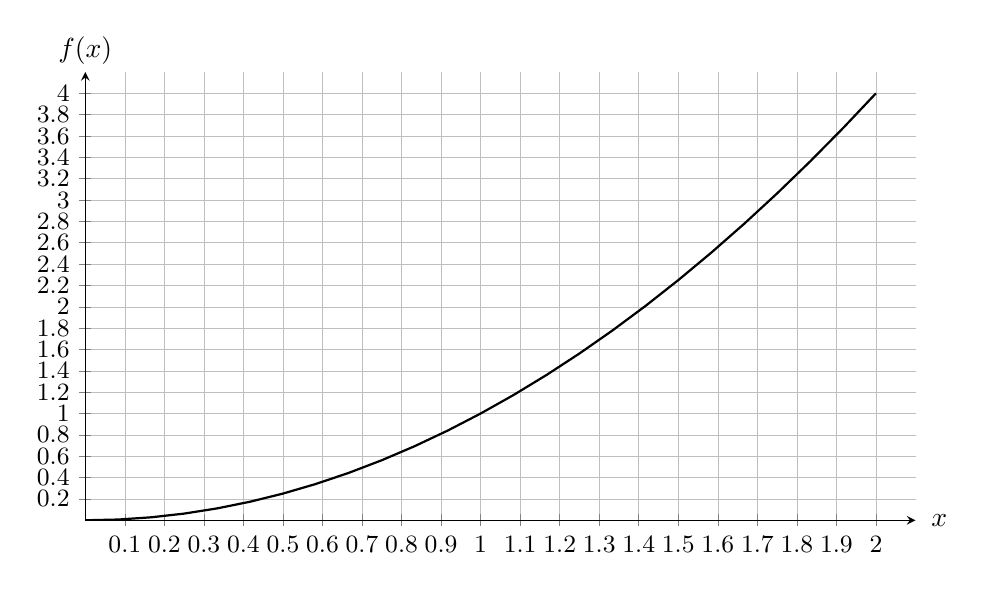
\begin{tikzpicture}
				\begin{axis}[
					grid = both,
					grid style={line width=.1pt, draw=gray!10},
					major grid style={line width=.2pt,draw=gray!50},
					width = \textwidth,
					height = .6\textwidth,
					every tick label/.append style={font=\small},
					axis x line = middle,
					axis y line = left,
		    			every axis y label/.style={at={(ticklabel cs:1.15)}},
						y label style={at={(axis description cs:0,1.1)},anchor=north},
					ytick = {0.2, 0.4,...,4},
		    			ylabel = {$f(x)$},
		    			ymin = 0, ymax = 4.2,
	    				every axis x label/.style= {at ={(ticklabel cs:1)}},
	    				xtick = {0.1, 0.2,...,2},
		    				x label style={at={(axis description cs:1.05,0)},anchor=east},
	    				xlabel = {$x$},
	    				xmin = 0, xmax = 2.1			
				]
					\addplot[thick, domain = 0:2] {x^2};
				\end{axis}
			\end{tikzpicture}\\[10pt]
			Approximate the slope of the tangent line to $f$ at $x = 1$ by finding the slope of the secant line through $(1,1)$ and the following points.  Sketch a few secant lines on the graph above as well.
			\begin{center}
			\begin{multicols*}{2}
				\begin{enumerate}[(a)]
					\setlength\itemsep{1.25in}
					\item $(0.7, 0.49)$
						
					\item $(0.8, 0.64)$
						 							
					\item $(0.9, 0.81)$
						\columnbreak
											
					\item $(1.3, 1.69)$
						 							
					\item $(1.2, 1.44)$
						 							
					\item $(1.1, 1.21)$

				\end{enumerate}
					\raggedcolumns
			\end{multicols*}
			\end{center}
		\end{ex}
			\newpage
			
	\subsubsection*{Pre-Class Activity}
	\addcontentsline{toc}{subsubsection}{Pre-Class Activity}
		\begin{ex}
			\begin{enumerate}[(a)]
				\item In Example 1.4.3, what happened to the slopes as you moved from (a) to (c), and from (d) to (f)?  Be descriptive.
					\vs{1}
					
				\item Example 2 does not give us an exact value for the tangent line.  How could we \emph{improve} the approximation we got?
					\vs{1}			
			\end{enumerate}
		\end{ex}
		\newsec
		
	\subsection*{In-Class}
	\addcontentsline{toc}{subsection}{In-Class}
		\begin{ex}
			Use a calculator to estimate the slope of the tangent line to the curve $f(x) = \sqrt{x}$ at $x = 3$.  Record your answers to 6 decimal places, and round your final answer to the hundredths place, if necessary.\\
		\begin{center}
				\begin{minipage}{.45\textwidth}
					\tabulinesep=1mm
					\begin{tabu}{|X[c]|X[1.5,c]|}\hline
						$x$ 		& $\dfrac{f(x) - f(3)}{x-3}$ \\ \hline
								& \\
						2.9		& \\ 
								& \\ \hline
								& \\
						2.99	& \\
								& \\ \hline 
								& \\
						2.999	& \\ 
								& \\ \hline
								& \\ 
						2.9999	& \\ 
								& \\ \hline
								& \\
						2.99999	&\\
								&\\ \hline\hline
								&\\
						Left-hand		& \\
						Slope $\approx$		&\\ \hline
					\end{tabu}
				\end{minipage}
				\begin{minipage}{.45\textwidth}
					\tabulinesep=1mm
					\begin{tabu}{|X[c]|X[1.5,c]|}\hline
						$x$ 		& $\dfrac{f(x) - f(3)}{x-3}$ \\ \hline
								& \\
						3.1		& \\ 
								& \\ \hline
								& \\
						3.01	& \\
								& \\ \hline 
								& \\
						3.001	& \\ 
								& \\ \hline
								& \\ 
						3.0001	& \\ 
								& \\ \hline
								& \\
						3.00001	&\\
								&\\ \hline\hline
								&\\
						Right-hand		& \\
						Slope $\approx$		&\\ \hline
					\end{tabu}
				\end{minipage}
					\vs{.3}
				\[\text{Slope at  }x = 3\approx \makebox[3in]{\hrulefill}\]
					
			\end{center}					
		\end{ex}	
			\newpage
			
	\subsubsection*{Velocity}
	\addcontentsline{toc}{subsubsection}{Velocity}

		Suppose we want to find the average velocity of an object.  We can use the same approach as we did above to find this.  The average velocity of an object is given by
			\[v_{avg} = \dfrac{\text{change in position}}{\text{change in time}}\]
			
		\begin{question}
			What connection might exist between $v_{avg}$ and the work we did in the previous exercises?
		\end{question}
			\vs{1}
			
		\begin{ex}
			Suppose a ball is dropped from the top of Dale Hall Tower, which is 250m tall.  Find the average velocity of the ball over the given intervals.  Use the fact  that free-fall of an object is given by the equation $s(t) = 4.9t^2$ m.  
			\begin{enumerate}[(a)]
				\item $[0,6]$
					\vs{1}
					
				\item $[2,5]$
					\vs{1}
					
				\item $[3,3.5]$
					\vs{1}
					
				\item $[3,3.01]$
					\vs{1}
					
				\item $[3,3.0001]$
					\vs{1}
					
			\end{enumerate}
		\end{ex}
			\newpage
			
		\begin{question}
			In Example 7, what do you think the purpose was of looking at so many average velocities?
		\end{question}
			\vs{1}
		
		\newsec
	\subsection*{After Class}
	\addcontentsline{toc}{subsection}{After Class}
		\begin{ex}
			The point $P = \lrpar{\dfrac{1}{2},0}$ lies on the curve $y = \cos \pi x$.
			\begin{enumerate}[(a)]
				\item If $Q$ is the point $(x,\cos \pi x)$, find the slope of the secant line $PQ$ (to six decimal places) for the following values of $x$.  Show your work, and make sure your calculator is in radian mode.
				\begin{enumerate}[(i)]
					\item 0.4
						\vs{.5}
					\item 0.49
						\vs{.5}
					\item 0.4999
						\vs{.5}
					\item 0.6
						\vs{.5}
					\item 0.51
						\vs{.5}
					\item 0.5001
						\vs{.5}
				\end{enumerate}
				\item Using part (a), estimate the value of the slope of the tangent line to $y$ at $x = 0.5$ to two decimal places.
					\vs{.5}
				\item Using part (b), find an equation for the tangent line to $y$ at $x = 0.5$.
					\vs{1}
			\end{enumerate}
		\end{ex}
			\newpage
			
		\begin{ex}
			If a rock is thrown upward on Io with a velocity of 10 m/s, its height (in meters) $t$ seconds later is given by $y = 10t - 1.86$.
			\begin{enumerate}[(a)]
				\item Find the average velocity over the given time intervals:
				\begin{enumerate}[(i)]
					\item $[1,2]$
						\vs{.5}
					\item $[1,1.5]$
						\vs{.5}
					\item $[1,1.1]$
						\vs{.5}
					\item $[1,1.01]$
						\vs{.5}
					\item $[1,1.001]$
						\vs{.5}
				\end{enumerate}
				\item Estimate the instantaneous velocity when $t = 1$.
					\vs{1}
			\end{enumerate}
		\end{ex}
		
		\begin{ex}
			Imagine you need to teach this section to a student in another section.  How would you explain the connection between tangent lines and secant lines to them?  Be descriptive!
		\end{ex}
			\vs{2}
	\clearpage
\end{document}